
% \VignetteIndexEntry{Plotting dendrograms and tree diagrams with ggplot}
% \VignettePackage{ggdendro}
% \VignetteKeyword{dendrogram}
% \VignetteKeyword{ggplot}


% Definitions
\newcommand{\ggdendro}{\texttt{ggdendro}}
\newcommand{\dendrodata}{\texttt{dendro\_data}}
\newcommand{\code}[1]{\texttt{#1}}
\newcommand{\ggplot}{\texttt{ggplot}}

\documentclass[10pt,oneside]{article}

\usepackage{Sweave}
\begin{document}
\pagestyle{empty}

\setlength{\baselineskip}{1.25em}
\setlength{\parskip}{0.5em}
\setlength{\parindent}{0.0em}

%\begin{titlepage}
\title{Using the \ggdendro{} package for plotting dendrograms and tree diagrams}
\author{Andrie de Vries}
%\end{titlepage}
\maketitle{}

\ggdendro{} is a package that makes it easy to extract dendrogram and tree diagrams into a data frame.  

\section{Introduction}

The \ggdendro{} package provides a general framework to extract the plot data for a dendrograms and tree diagrams.

It does this by providing generic function \dendrodata{} that will extract the appropriate segment data as well as labels.  This data is returned as a list of data.frames.  These data frames can be extracted using three accessor functions:

\begin{itemize}
\item \code{segment}
\item \code{label}
\item \code{leaf\_label}
\end{itemize}

The package also provides two convenient wrapper functions:

\begin{itemize}
\item\code{ggdendrogram} is a wrapper around \ggplot{} to create a dendrogram using a single line of code.  The resulting object is of class \ggplot{}, so can be manipulated using the \ggplot{} tools.
\item\code{theme\_dendro} is a \ggplot{} theme with a blank canvas, i.e. no axes, axis labels or tick marks.
\end{itemize}

The \code{ggplot} package doesn't get loaded automatically, so remember to load it first: 
  
\begin{Schunk}
\begin{Sinput}
> library(ggplot2)
> library(ggdendro)
\end{Sinput}
\end{Schunk}

%------------------------------------------------------------------------------
\section{Using the \code{ggdendrogram} wrapper}

The \ggdendro{} package will extract all of the plot data from dendrogram objects.  Sometimes it is useful to have fine-grained control over the plot.  Other times it might be more convenient to have a simple wrapper around \code{ggplot} to produce a dendrogram with a small amount of code.

The function \code{ggdendrogram} provides such a wrapper to produce a plot with a single line of code.  It provides a few options for controlling the display of line segments, labels and plot rotation (rotated by 90 degrees or not).  

\begin{Schunk}
\begin{Sinput}
> hc <- hclust(dist(USArrests), "ave")
> p <- ggdendrogram(hc, rotate=FALSE, size=2)
> print(p)
\end{Sinput}
\end{Schunk}

\begin{figure}[h]
\begin{center}
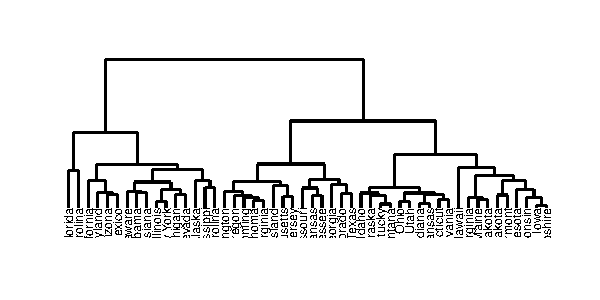
\includegraphics[width=4in, height=2in]{ggdendro-dendrogram}
\end{center}
\caption{A dendrogram produced using \code{ggdendrogram}}
\end{figure}

The next section shows how to take full control over the data extraction and subsequent plotting.

%------------------------------------------------------------------------------
\section{Extracting the dendrogram plot data using \dendrodata{}}

The \code{hclust} and \code{dendrogram} functions in R makes it easy to plot the results of hierarchical cluster analysis and other dendrograms in R.  However, it is hard to extract the data from this analysis to customise these plots, since the \code{plot} functions for both these classes prints directly without the option of returning the plot data.  

\begin{Schunk}
\begin{Sinput}
> hc <- hclust(dist(USArrests), "ave")
> dhc <- as.dendrogram(hc)
> # Rectangular lines
> ddata <- dendro_data(dhc, type="rectangle")
> p <- ggplot(segment(ddata)) + 
+     geom_segment(aes(x=x0, y=y0, xend=x1, yend=y1)) + 
+     coord_flip() + scale_y_reverse(expand=c(0.2, 0))
> print(p)
\end{Sinput}
\end{Schunk}

\begin{figure}[h]
\begin{center}
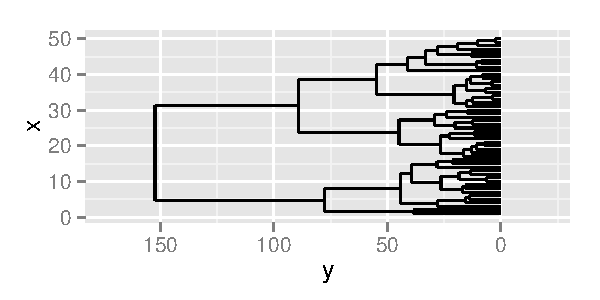
\includegraphics[width=4in, height=2in]{ggdendro-dendro1}
\end{center}
\caption{A dendrogram produced using \dendrodata{} and \code{ggplot}}
\end{figure}


Of course, using ggplot to create the dendrogram means one has full control over the appearance of the plot.  For example, here is the same data, but this time plotted horizontally with a clean background.  In \code{ggplot} this means passing a number of options to \code{opts}.  \ggdendro{} has a convenient function, \code{theme\_dendro} that wraps these options into a convenient function.

\begin{Schunk}
\begin{Sinput}
> p <- p + coord_flip() + theme_dendro()
> print(p)
\end{Sinput}
\end{Schunk}

\begin{figure}[h]
\begin{center}
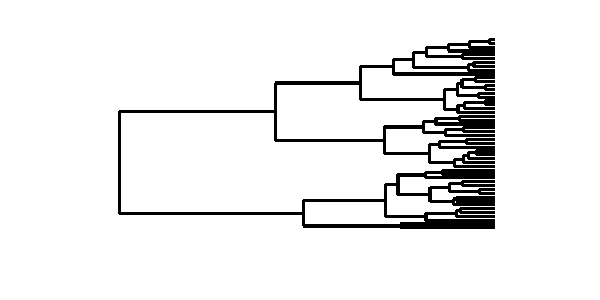
\includegraphics[width=4in, height=2in]{ggdendro-dendro2}
\end{center}
\caption{Dendrogram rotated on clear background}
\end{figure}

Dendrograms can also be drawn using triangular lines instead of rectangular lines.  For example:

\begin{Schunk}
\begin{Sinput}
> ddata <- dendro_data(dhc, type="triangle")
> p <- ggplot(segment(ddata)) + 
+     geom_segment(aes(x=x0, y=y0, xend=x1, yend=y1)) + 
+     coord_flip() + scale_y_reverse(expand=c(0.2, 0)) +
+     theme_dendro()
> print(p)
\end{Sinput}
\end{Schunk}

\begin{figure}[h]
\begin{center}
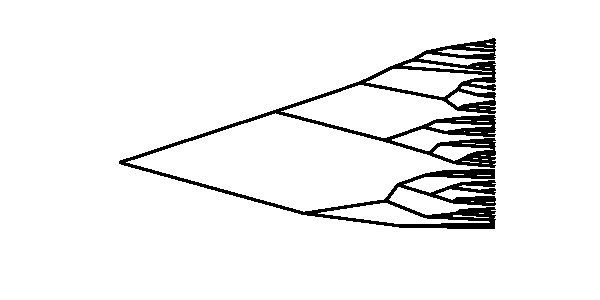
\includegraphics[width=4in, height=2in]{ggdendro-dendro3}
\end{center}
\caption{A dendrogram with triangular connection lines}
\end{figure}

  

%------------------------------------------------------------------------------
\section{Regression tree diagrams}

The \code{tree} function in package \code{tree} creates tree diagrams.  To extract the plot data for these diagrams using \ggdendro{} follows the same basic pattern as dendrograms: 

\begin{Schunk}
\begin{Sinput}
> require(tree)
> data(cpus, package="MASS")
> cpus.ltr <- tree(log10(perf) ~ 
+         syct+mmin+mmax+cach+chmin+chmax, cpus)
> tree_data <- dendro_data(cpus.ltr)
> p <- ggplot(segment(tree_data)) +
+     geom_segment(aes(x=x, y=y, xend=xend, yend=yend, size=n), 
+         colour="blue", alpha=0.5) +
+     scale_size("n", to=c(0, 3)) +
+     geom_text(data=label(tree_data), 
+         aes(x=x, y=y, label=label), vjust=-0.5, size=3) +
+     geom_text(data=leaf_label(tree_data), 
+         aes(x=x, y=y, label=label), vjust=0.5, size=2) +
+     theme_dendro()
> print(p)
\end{Sinput}
\end{Schunk}

\begin{figure}[h]
\begin{center}
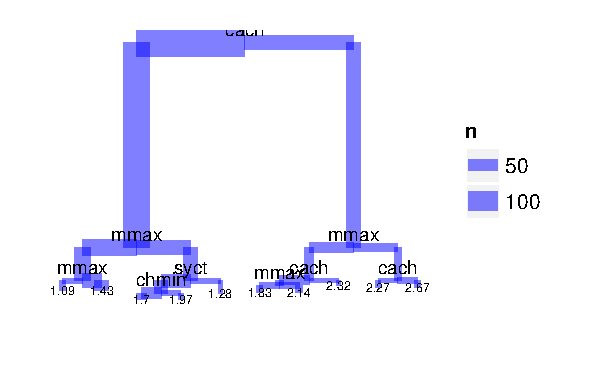
\includegraphics[width=4in, height=2.5in]{ggdendro-tree1}
\end{center}
\caption{Regression tree plot}
\end{figure}


%------------------------------------------------------------------------------
\section{Classification tree diagrams}

The \code{rpart} function in package \code{rpart} creates classification diagrams.  To extract the plot data for these diagrams using \ggdendro{} follows the same basic pattern as dendrograms: 

\begin{Schunk}
\begin{Sinput}
> fit <- rpart(Kyphosis ~ Age + Number + Start, 
+     method="class", data=kyphosis)
> fitr <- dendro_data(fit)
> p <- ggplot() + 
+     geom_segment(data=fitr$segments, 
+         aes(x=x, y=y, xend=xend, yend=yend)) + 
+     geom_text(data=fitr$labels, 
+         aes(x=x, y=y, label=label), size=3, vjust=0) +
+     geom_text(data=fitr$leaf_labels, 
+         aes(x=x, y=y, label=label), size=3, vjust=1) +
+     theme_dendro()
> print(p)
\end{Sinput}
\end{Schunk}

\begin{figure}[h]
\begin{center}
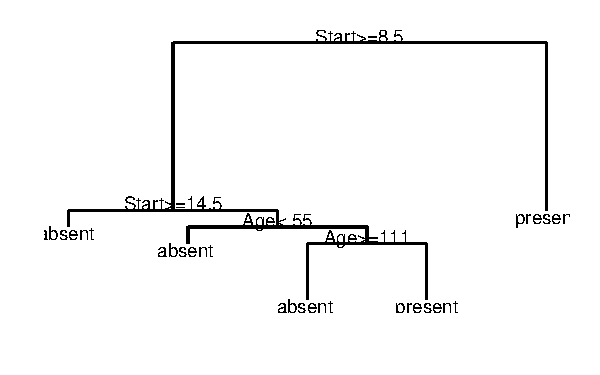
\includegraphics[width=4in, height=2.5in]{ggdendro-rpart1}
\end{center}
\caption{Classification tree plot}
\end{figure}


%------------------------------------------------------------------------------
\section{Conclusion}

The \ggdendro{} package makes it easy to extract the line segment and label data from hclust, dendrogram and tree objects.


% Start a new page
% Not echoed, not evaluated
% ONLY here for checkVignettes so that all output doesn't
% end up on one enormous page

\end{document}




